\section{Sprung}
Das Zeitverhalten der 3 Tiefpässe soll an Hand der Sprungantworten untersucht werden. Zur Messung der Sprungantwort wird das Filter mit einem periodischen Rechtecksignal geeigneter Amplitude und Frequenz aus einem Funktionsgenerator angesteuert und das Ausgangssignal auf dem Oszilloskop abgebildet.
 Skizzieren Sie die Messschaltung mit Angabe der verwendeten Geräte und plotten Sie Einund Ausgangssignale für die drei Tiefpässe. Bestimmen Sie aus den Sprungantworten der drei Tiefpässe Anstiegszeit, Überschwingen (bezogen auf Endwert) und Einschwingzeit (bezogen auf 5% Abweichung vom Endwert) und stellen Sie alle Werte in einer Tabelle gemeinsam dar!


%%%%%%%%%%%%%%%%%%%%%%%%%%%%%%%%%%%%%%%%%%%%%%%%Comments
%Plots der Sprungantworten der drei Tiefpässe, Bestimmung von Anstiegszeit, Überschwingen und Einschwingzeit; Darstellung und Vergleich in einer Tabelle
%multi figure
\begin{figure}[H]
\begin{center}
\subfloat[\imgfilename]{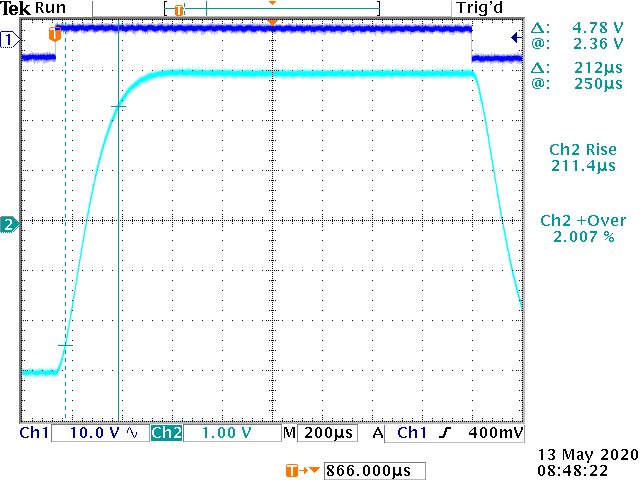
\includegraphics[width = \textwidth/3]{img/4 Bessel Anstiegszeit.png}}  
\subfloat[\imgfilename]{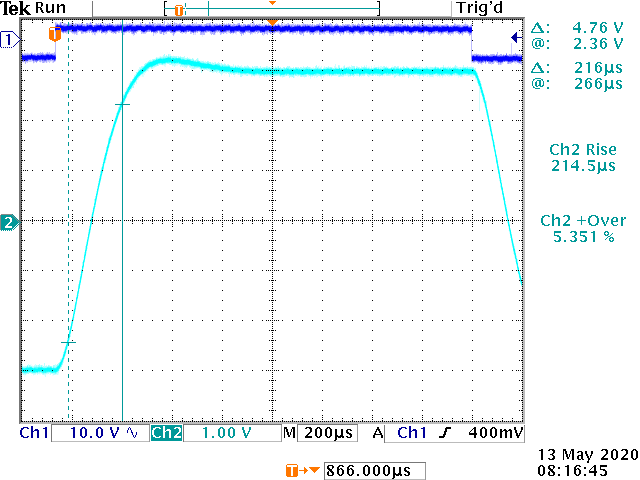
\includegraphics[width = \textwidth/3]{img/4 Butterworth Anstiegszeit .png}} 
\subfloat[\imgfilename]{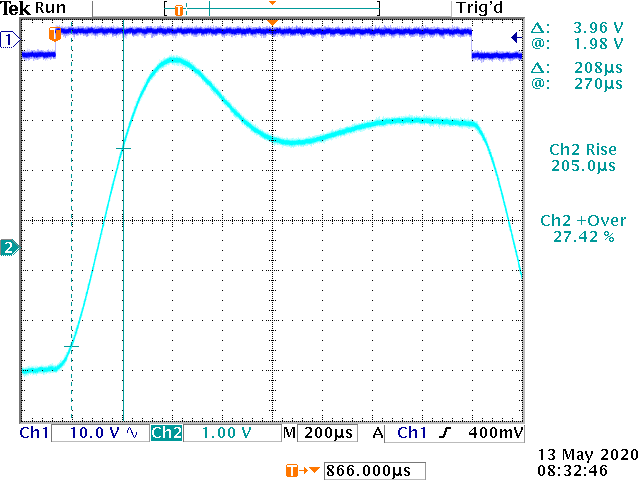
\includegraphics[width = \textwidth/3]{img/4 Tscheby Anstiegszeit.png}} \\
\subfloat[\imgfilename]{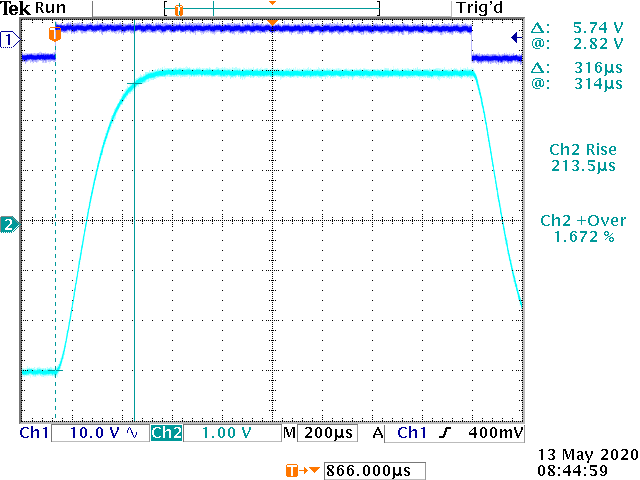
\includegraphics[width = \textwidth/3]{img/4 Bessel Einschwingzeit.png}}  
\subfloat[\imgfilename]{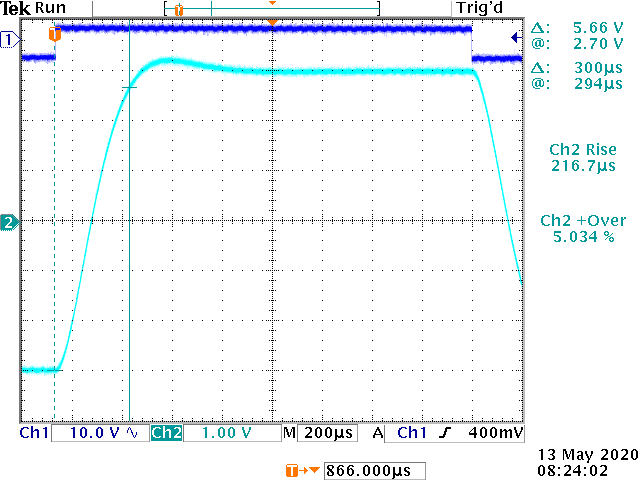
\includegraphics[width = \textwidth/3]{img/4 Butterworth Einschwingzeit.png}} 
\subfloat[\imgfilename]{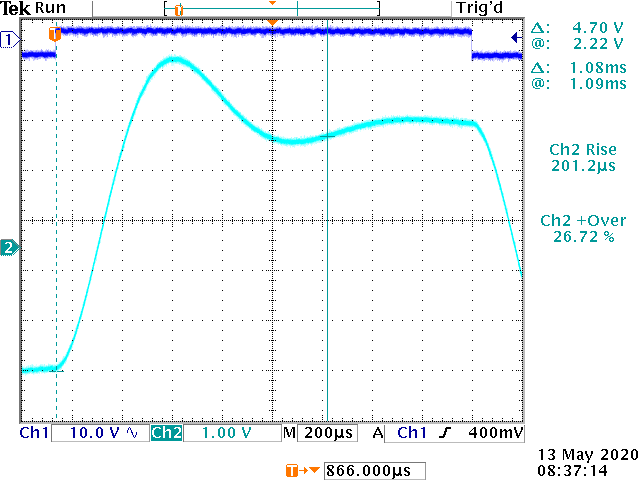
\includegraphics[width = \textwidth/3]{img/4 Tscheby Einschwingzeit.png}} \\
\subfloat[\imgfilename]{\includegraphics[width = \textwidth/3]{img/4 Bessel Überschwingzeit.png}}  
\subfloat[\imgfilename]{\includegraphics[width = \textwidth/3]{img/4 Butterworth Überschwingen}} 
\subfloat[\imgfilename]{\includegraphics[width = \textwidth/3]{img/4 Tscheby Überschwingzeit}} \\
\caption{Anstiegszeit, Einschwingzeit und Überschwingzeit}
\label{fig:A4_mult}
\end{center}
\end{figure}

\begin{table}[H]
    \centering
    \begin{tabular}{|c|c|c|c|c|}\hline
    \tbf{Filter} & \tbf{Anstiegszeit} & \tbf{Überschwingen}     &  \tbf{Einschwingen}     & \tbf{Ausgangsamplitude}   \\ \hline
    Butterworth                   & \SI{216}{\micro\second} &     \SI{0.26}{\volt} &\SI{300}{\micro\second} & \SI{6}{\volt_{pp}}   \\
    Tschebyscheff             & \SI{208}{\micro\second}  &    \SI{1.2}{\volt}  &\SI{1.08}{\milli\second} & \SI{5}{\volt_{pp}}   \\ 
    Bessel                &\SI{212}{\micro\second}  & \SI{40}{\milli\volt} &\SI{316}{\micro\second} &\SI{6}{\volt_{pp}} \\ \hline
    \end{tabular}
    \caption{Grenzfrequenzen der Filter}
\end{table}